\pdfminorversion=7
\documentclass[final,3p,times]{elsarticle}

\usepackage[T1]{fontenc}
\usepackage[utf8]{inputenc}
\usepackage{amsmath,amssymb}
\usepackage{booktabs}
\usepackage{threeparttable}
\usepackage{tabularx}
\usepackage{array}
\usepackage{makecell}
\usepackage{float}
\usepackage[section]{placeins}
\usepackage{url}
\usepackage{graphicx}
\usepackage[colorlinks=true,linkcolor=blue,citecolor=blue,urlcolor=blue]{hyperref}

\graphicspath{{fig/}{../artifacts/publication/figures/}{../artifacts/publication/diagnostics/}}
\sloppy
\newcommand{\stdfigure}[1]{\includegraphics[width=\linewidth,height=0.72\textheight,keepaspectratio]{#1}}

\journal{Applied Energy}

\begin{document}

\begin{frontmatter}

\title{Policy Learning with Surrogate Approximators for Block-Scale Urban Morphology Design: A Comparative Benchmarking Study}

\author[label1]{Haolin Wang}
\author[label1]{Zhi Wu\corref{cor1}}
\ead{zwu@seu.edu.cn}
\author[label1]{Wei Gu}
\author[label2]{Pengxiang Liu}
\author[label3]{Qirun Sun}
\author[label4]{Wei Wang}

\cortext[cor1]{Corresponding author.}

\affiliation[label1]{organization={School of Electrical Engineering, Southeast University},
            city={Nanjing},
            postcode={210096},
            country={China}}

\affiliation[label2]{organization={Department of Data Science, City University of Hong Kong},
            addressline={83 Tat Chee Avenue},
            city={Hong Kong Special Administrative Region of China},
            country={China}}

\affiliation[label3]{organization={School of Energy and Electrical Engineering, Hohai University},
            city={Nanjing},
            state={Jiangsu},
            postcode={211100},
            country={China}}

\affiliation[label4]{organization={School of Architecture, Southeast University},
            city={Nanjing},
            postcode={210096},
            country={China}}

\begin{abstract}
Integrating urban morphology generation, performance prediction, and design search is essential for low-carbon urban design, yet full simulation-based optimization remains computationally demanding. This study develops and evaluates a surrogate-assisted deep reinforcement learning (DRL) workflow for block-scale urban morphology design under surrogate-predicted energy indicators. A deep neural network (DNN) surrogate predicts Energy Use Intensity (EUIt), Energy Generation (EG), and Sunlight Hours (H) from 12 morphological factors, and a Deep Deterministic Policy Gradient (DDPG) agent searches the design space under different reward preferences. In the retained publication archives, the DDPG scenarios achieve stronger mean objective summaries than the NSGA-II archive and also attain a larger Hypervolume, while NSGA-II retains a lower IGD. The three reward settings nevertheless produce only modest separation in objective space, although they still yield interpretable morphology-level differences. Independent re-evaluation remains surrogate-bound and indicates larger discrepancies for the selected DDPG candidate than for the selected NSGA-II candidate. Overall, the proposed framework is better interpreted as a preference-conditioned region-finding and design-support tool than as a universally dominant replacement for Pareto-based evolutionary search.
\end{abstract}

\begin{keyword}
Multi-objective optimization \sep Urban morphology \sep Energy performance \sep Deep reinforcement learning
\end{keyword}

\end{frontmatter}

\section*{Abbreviations and Symbols}
\small
\noindent
\begin{minipage}[t]{0.48\linewidth}
\textbf{Abbreviations}

\begin{tabularx}{\linewidth}{@{}>{\raggedright\arraybackslash}p{0.24\linewidth}X@{}}
UM & Urban morphology \\
EP & Energy performance \\
UMF & Urban morphological factor \\
EPI & Energy performance indicator \\
DRL & Deep reinforcement learning \\
DNN & Deep neural network \\
DDPG & Deep Deterministic Policy Gradient \\
MOO & Multi-objective optimization \\
HV & Hypervolume \\
IGD & Inverted Generational Distance \\
\end{tabularx}
\end{minipage}\hfill
\begin{minipage}[t]{0.48\linewidth}
\textbf{Main symbols}

\begin{tabularx}{\linewidth}{@{}>{\raggedright\arraybackslash}p{0.28\linewidth}X@{}}
EUIt & Energy use intensity (kWh/m$^2$/y) \\
EG & Energy generation ($10^6$ kWh/y) \\
H & Sunlight hours (h) \\
FAR & Floor area ratio \\
BD & Building density \\
OSR & Open space ratio \\
SVF & Sky view factor \\
AF & Average floors \\
OSLI & Open Space Location Index \\
$\theta$ & Block orientation angle (deg) \\
$w_1,w_2,w_3$ & Reward weights for EUIt, EG, and H \\
$\gamma$, $\tau$ & DDPG discount and soft-update factors \\
\end{tabularx}
\end{minipage}
\normalsize

\section{Introduction}

In the context of carbon peaking and carbon neutrality, deep decarbonization of urban energy systems has become a central issue in sustainable development \cite{ref1,ref2}. Because cities concentrate both energy demand and renewable-energy opportunities, urban morphology (UM) has a strong influence on building energy performance (EP), solar access, and environmental quality \cite{ref3,ref4,ref5}. However, urban design and energy planning are still often treated as separate tasks in practice, which weakens the energy performance of block-scale development and limits the effective use of renewable resources \cite{ref6,ref7}. Developing an integrated framework that links morphology generation, performance evaluation, and design optimization is therefore an important research problem at the intersection of architecture, urban planning, and energy systems \cite{ref8}.

This context also highlights the methodological importance of surrogate-based design studies. In practice, large comparative sweeps over urban-energy design strategies are often bottlenecked by expensive simulation workflows, so surrogate-assisted optimization is increasingly used as a screening layer before full physical validation. Under these conditions, optimizer reliability becomes part of the energy-design problem itself: if a learning-based method is unstable, checkpoint-sensitive, or difficult to benchmark fairly, its practical value for urban energy design is limited.

\subsection{Research Motivation}

To address this challenge, computational design methods based on parametric modeling and multi-objective optimization (MOO) have become mainstream \cite{ref9,ref10}. Evolutionary algorithms, exemplified by NSGA-II, are widely used to explore the design space and identify Pareto-optimal trade-offs among conflicting objectives such as energy consumption \cite{ref11}, energy generation potential \cite{ref12}, and daylighting \cite{ref13}. However, this search-oriented paradigm frames urban morphology design primarily as Pareto-front exploration in a high-dimensional, nonlinear, and strongly coupled design space.

The core motivation of this study is therefore to test whether a preference-conditioned policy-learning formulation can identify stable high-performing surrogate regions and interpretable morphology patterns under a shared optimization budget. Rather than assuming that policy learning should dominate Pareto search, this study asks whether it offers a useful alternative inductive bias for navigating the same surrogate landscape.

\subsection{Literature Review and Research Gap}

The mainstream approach for multi-objective optimization in urban design relies on search-based algorithms \cite{ref14,ref15}, particularly evolutionary algorithms such as NSGA-II \cite{ref16}. These methods primarily explore complex problem spaces to identify trade-off solutions among conflicting metrics, such as energy efficiency and cost \cite{ref17}. Despite their widespread adoption, this search-centric paradigm faces three fundamental limitations.

First, the computational cost is high. Evolutionary algorithms require repeated performance evaluations of large numbers of design candidates, and simulations based on engines such as EnergyPlus are inherently time-consuming \cite{ref18,ref19}. As design-space dimensionality increases, the time required to identify a convergent Pareto front can extend from several days to weeks \cite{ref20}.

Second, evolutionary algorithms inherently operate as black-box models \cite{ref21}. Their search operators emphasize archive quality and diversity, but they do not directly provide a reusable policy for preference-conditioned navigation of the design space. As a result, designers are often presented with a cloud of Pareto-optimal solutions from which it is difficult to derive interpretable and transferable design strategies \cite{ref22,ref23}.

Third, the mechanisms of NSGA-II are designed to preserve diversity and delineate the boundary of the Pareto front \cite{ref24}. By contrast, a scalarized policy-learning formulation can concentrate repeated search on a narrower surrogate region. Whether such concentration reveals robust design patterns or merely amplifies surrogate bias must be tested empirically rather than assumed a priori \cite{ref25}.

To overcome these limitations, this study adopts Deep Reinforcement Learning (DRL) as an alternative optimization paradigm \cite{ref26}. DRL combines the nonlinear feature representation capability of deep learning with the sequential decision-making framework of reinforcement learning. Instead of conducting blind searches, the agent learns a policy through repeated interaction with the environment. DRL has achieved considerable success in complex, high-dimensional decision tasks such as robotic control \cite{ref27}, strategy games \cite{ref28}, natural language processing \cite{ref29}, and autonomous driving \cite{ref30}.

These tasks share a core challenge: sequential decision-making in high-dimensional, continuous state and action spaces. This challenge mirrors urban morphology optimization, where designers must determine 12 continuously variable morphological factors. Because value-function methods such as DQN \cite{ref31} are designed for discrete actions, this study focuses on the Deep Deterministic Policy Gradient (DDPG) algorithm. DDPG \cite{ref32}, an actor-critic method for continuous control, provides a simple and interpretable baseline for policy learning in continuous design spaces. We do not claim that DDPG is universally optimal relative to alternatives such as TD3, SAC, PPO with continuous actions, CMA-ES, MOEA/D, or Bayesian optimization. Rather, the goal of this study is to examine whether a preference-conditioned policy-learning formulation can yield useful design strategies under a shared surrogate environment.

Although DRL shows substantial promise, its application to the interdisciplinary problem of urban morphology design with surrogate energy indicators remains largely unexplored. While DRL is increasingly used for building energy control \cite{ref33,ref34} and energy system operation \cite{ref35,ref36}, its use as a design-space navigation tool for urban morphology is still nascent. In particular, its behavior relative to a benchmark such as NSGA-II has not yet been rigorously characterized under a shared surrogate environment.

\subsection{Study Contributions and Paper Structure}

Against this background, this study develops and evaluates a DRL-DNN integrated framework for block-scale urban morphology design. Three specialist agents with distinct reward preferences are trained and compared with an NSGA-II benchmark under the same surrogate environment.

\begin{enumerate}
\item This study develops a DRL-DNN framework for urban morphology design by transforming the search problem into a reward-weighted policy-learning task under a shared surrogate environment.
\item This study examines whether different reward priorities lead to distinguishable search tendencies and morphology signatures within the same surrogate landscape.
\item This study compares DRL and NSGA-II under a shared surrogate environment using both Pareto-quality metrics and preference-aligned objective summaries.
\item This study combines linear correlation analysis with nonlinear response diagnostics to interpret how key UMFs influence EUIt, EG, and H.
\end{enumerate}

The remainder of this paper is organized as follows. Section~2 presents the DRL-DNN integrated framework, including parametric modeling, performance simulation, surrogate modeling, and the DDPG optimization engine. Section~3 reports the experimental results and comparative analysis. Section~4 discusses the implications and limitations of the study. Section~5 concludes the paper. Additional case-setting and surrogate-validation details are provided in Appendix~A, and benchmark-robustness diagnostics are reported in Appendix~B.

\section{Methodology}

This study proposes an integrated surrogate-assisted workflow for block-scale urban morphology design. As illustrated in Fig.~1, the framework combines parametric morphology generation, performance simulation, surrogate modeling, and policy learning. A parametric dataset is first constructed to link urban morphological factors (UMFs) with key energy performance indicators (EPIs). A DNN surrogate is then trained for rapid performance prediction, after which a DDPG agent interacts with the surrogate environment to search for morphology strategies that balance energy demand, energy generation, and sunlight access.

\begin{figure}[H]
\centering
\stdfigure{fig1}
\caption{Overview of the proposed method. The left block summarizes parametric morphology generation and performance simulation, while the right block shows the surrogate-assisted optimization workflow used during policy learning.}
\label{fig:overview}
\end{figure}

\subsection{Case Study and Parametric Modeling}

The selected research area is Jianhu County, located in Jiangsu Province in the eastern coastal region of China. The county is situated between $33^\circ16'$ and $33^\circ41'$ N latitude and $119^\circ33'$ and $120^\circ05'$ E longitude, with an average elevation of 2~m. It has an administrative area of approximately 1160~km$^2$ and a population of around 600,000, resulting in a population density of about 520 persons/km$^2$. According to the Chinese Code for Thermal Design of Civil Buildings, Jianhu lies within the hot-summer and cold-winter climate zone and is classified as having a humid subtropical climate under the Koppen-Geiger system. The climate necessitates both building heating and cooling, as the average dry-bulb temperature is $27.1^\circ$C in the hottest month (July) and $1.6^\circ$C in the coldest month (January), with an annual average of $15.0^\circ$C. Furthermore, the region presents favorable conditions for solar energy utilization, receiving annual solar radiation of about 1250~kWh/m$^2$ and approximately 1800 hours of sunshine per year.

To generate a diverse dataset linking urban form to energy performance, a parametric modeling approach was implemented on the Grasshopper platform. The core of this approach involves defining a standard urban block subdivided into a $3\times3$ grid, creating nine land units. Based on an analysis of the existing urban fabric, a set of representative residential building prototypes, such as point, slab, and courtyard types, were defined. In the parametric model, one land unit is designated as open space, while the remaining eight units are populated with these building prototypes to generate a wide variety of block morphologies.

This parametric generation process is controlled by twelve selected UMFs. These include Floor Area Ratio (FAR), Building Density (BD), Open Space Ratio (OSR), Average Floors (AF), Setback Diversity (SD), Shape Coefficient (SC), Average Perimeter-to-Area Ratio (PAR), Aspect Ratio (AR), average Sky View Factor (SVF), Open Space Location Index (OSLI), and Block Orientation Angle $\theta$. Once the geometric model of the block is configured on the Grasshopper platform, these UMFs can be calculated using its built-in tools. In the present dataset, 500 generated morphologies are used for surrogate training and validation; this sample size is sufficient for an initial regression study but remains limited relative to the full 12-dimensional continuous design space. The formulas used in this work are summarized in Table~\ref{tab:umf}.

\begin{table}[H]
\caption{Calculation formulas of the morphological factors.}
\label{tab:umf}
\centering
\footnotesize
\begin{threeparttable}
\begin{tabularx}{0.92\linewidth}{@{}>{\centering\arraybackslash}p{0.17\linewidth} >{\centering\arraybackslash}p{0.16\linewidth} >{\centering\arraybackslash}X@{}}
\toprule
Factor & Symbol & Formula \\
\midrule
Floor area ratio & FAR & $\mathrm{FAR}=\dfrac{\sum_{i=1}^{n} S_i}{A_s}$ \\
Setback diversity & SD & $\mathrm{SD}=h_{\max}-h_a$ \\
Average floors & AF & $\mathrm{AF}=\dfrac{\sum_{i=1}^{n} S_i}{\sum_{i=1}^{n} f_i}$ \\
Aspect ratio & AR & $\mathrm{AR}=\dfrac{1}{n}\sum_{i=1}^{n}\dfrac{H_i}{W_i}$ \\
Sky view factor & SVF & $\mathrm{SVF}=\dfrac{1}{2\pi}\int_{0}^{2\pi}\cos^2\!\bigl(\beta(R,\theta)\bigr)\,d\theta$ \\
Building density & BD & $\mathrm{BD}=\dfrac{\sum_{i=1}^{n} f_i}{A_s}$ \\
Open space ratio & OSR & $\mathrm{OSR}=\dfrac{A_s-\sum_{i=1}^{n} f_i}{\sum_{i=1}^{n} S_i}$ \\
Shape coefficient & SC & $\mathrm{SC}=\dfrac{\sum_{i=1}^{n} c_i}{\sum_{i=1}^{n} h_i f_i}$ \\
Perimeter-to-area ratio & PAR & $\mathrm{PAR}=\dfrac{\sum_{i=1}^{n} p_i}{\sum_{i=1}^{n} f_i}$ \\
\bottomrule
\end{tabularx}
\begin{tablenotes}[flushleft]
\footnotesize
\item Note: $n$ is the number of buildings; $OR_i$ is the orientation of building $i$; $S_i$ is the total floor area of building $i$; $A_s$ is the block area; $f_i$ is the floor area of building $i$; $h_{\max}$ and $h_a$ are the maximum and average building heights of the block; $H_i$ and $W_i$ describe the height and width difference of the canyon; $c_i$ is the surface area of building $i$; $p_i$ is the perimeter of building $i$; and $\beta$ is the angle from the center point to the maximum obstacle height at a distance equal to the constant search radius $R$.
\end{tablenotes}
\end{threeparttable}
\end{table}

In addition to the factors in Table~\ref{tab:umf}, OSLI is introduced to characterize the topological position of the open space within the $3\times3$ grid and to account for its influence on local wind, thermal, and daylight conditions \cite{ref17,ref18}. OSLI is an integer variable ranging from 0 to 8. Furthermore, the block orientation angle $\theta$, ranging from $[-45^\circ,45^\circ]$, is included to regulate solar access. Additional geometric details of the block layout and the representative building prototypes are provided in Appendix~A.

\subsection{Performance Simulation and Optimization Objectives}

This study evaluates the energy behavior and solar potential of residential blocks using three key EPIs: total Energy Use Intensity (EUIt), Energy Generation (EG), and Sunlight Hours (H). Together, these indicators capture the demand, supply, and daylight dimensions of block-scale energy performance.

H, which indicates the duration of solar radiation exposure, was simulated using the Sunlight Hours Analysis module in Ladybug for a typical coldest day (January~20, 08:00--16:00). Continuous test points were set at 1~m intervals along south-facing ground-floor windowsills 0.9~m above ground, and the Radiance engine calculated solar trajectories and shading. The average sunlight hours across all test points represent the overall daylighting performance of the block.

EUIt, a core indicator of energy-saving performance, was simulated by constructing a Honeybee energy model based on EnergyPlus, with parameters set according to Chinese standards JGJ~134-2010 and GB~50736-2012. The simulation applied a stratified thermal zoning strategy, set the building function uniformly to residential, and used the Urban Weather Generator (UWG) to convert standard weather data into urban microclimate data to account for the urban heat island effect.

EG, representing the block's renewable-energy potential, was calculated from annual rooftop solar radiation using a coupled Ladybug-Radiance simulation. The model assumes a polycrystalline silicon PV system with 17\% efficiency and 85\% DC/AC conversion under standardized conditions, including 90\% roof coverage and $0^\circ$ tilt, to ensure comparability across cases. PV potential was then assessed against a threshold of 800~kWh/m$^2$/year. Finally, a Dragonfly-Ladybug toolchain was used to automate geometric information extraction and parameter transfer, thereby ensuring spatial consistency across all simulation models.

\begin{table}[H]
\caption{Parameters and settings for the building energy simulation in EnergyPlus.}
\label{tab:energyplus}
\centering
\footnotesize
\begin{threeparttable}
\begin{tabularx}{0.94\linewidth}{@{}>{\centering\arraybackslash}p{0.23\linewidth} >{\centering\arraybackslash}p{0.24\linewidth} >{\centering\arraybackslash}X@{}}
\toprule
Classification & Parameter & Specification \\
\midrule
System settings & Weather data & EPW files modified based on UWG urban microclimate simulations \\
System settings & Simulation period & Annual simulation (January~1 to December~31) \\
Envelope thermal performance & Wall U-value & 0.8~W/(m$^2\cdot$K) \\
Envelope thermal performance & Roof U-value & 0.5~W/(m$^2\cdot$K) \\
Envelope thermal performance & Floor U-value & 1.5~W/(m$^2\cdot$K) \\
Envelope thermal performance & Window properties & U-value = 2.70~W/(m$^2\cdot$K); Solar Heat Gain Coefficient (SHGC) = 0.78 \\
Window-to-wall ratio & North \& South facades & 0.4 \\
Window-to-wall ratio & East \& West facades & 0.1 \\
Internal loads & Occupant density & 0.03 persons/m$^2$; metabolic rate = 100~W/person \\
Internal loads & Lighting power density & 5~W/m$^2$ \\
Internal loads & Equipment power density & 1.9~W/m$^2$ \\
Internal loads & Ventilation rate & 30~m$^3$/(h$\cdot$person) \\
HVAC system & Thermostat setpoints & Heating: Dec~1--Feb~28, $18^\circ$C; Cooling: Jun~15--Aug~31, $26^\circ$C \\
HVAC system & Infiltration rate & 1~ACH (natural air leakage) \\
\bottomrule
\end{tabularx}
\end{threeparttable}
\end{table}

\subsection{DNN-based Surrogate Model}

In this study, a DNN is constructed as a predictive surrogate model to estimate the three target performance indicators from the simulated dataset. The model adopts a multi-layer feedforward architecture in which information flows from the input layer through the hidden layers to the output layer. Through stacked fully connected transformations, the network captures the nonlinear relationships between urban morphological factors and block-scale performance outcomes.

The DNN training process consists of two key stages: forward propagation and backpropagation. In the forward stage, the network processes input data to generate a prediction. During backpropagation, the prediction error is propagated backward from the output layer to the input layer. This process involves calculating the gradient of the loss function with respect to the network weights and iteratively updating the model parameters to reduce prediction error:

\begin{equation}
\mathbf{w} = \mathbf{w} + \eta \nabla_{\mathbf{w}} = \mathbf{w} + \eta\,\mathrm{backpropagation}\!\left(f(\mathbf{x})\right),
\end{equation}

where $\eta$ is the learning rate and $f(\mathbf{x})$ is the objective function to minimize.

To determine the DNN architecture and training settings, Bayesian Optimization (BO) was used for automated hyperparameter tuning. Compared with grid search, BO guides the search process by constructing a probabilistic model of the objective function and repeatedly selecting promising hyperparameter combinations. After the optimal settings were determined, model performance was evaluated using five-fold cross-validation. Because the surrogate is subsequently used for optimization, it is treated here as an optimization-enabling approximation rather than as a direct replacement for the original simulation workflow.

\begin{table}[H]
\caption{Optimal hyperparameters of the DNN determined by Bayesian Optimization.}
\label{tab:dnn-hyper}
\centering
\footnotesize
\begin{threeparttable}
\begin{tabularx}{0.62\linewidth}{@{}>{\centering\arraybackslash}X>{\centering\arraybackslash}X@{}}
\toprule
Hyperparameter & Value \\
\midrule
Number of dense layers & 2 \\
Units of 1st layer & 64 \\
Units of 2nd layer & 32 \\
Dropout rate & 0.2 \\
Learning rate & 0.001 \\
Batch size & 32 \\
Optimizer & Adam \\
Activation & ReLU \\
\bottomrule
\end{tabularx}
\end{threeparttable}
\end{table}

To ensure a rigorous evaluation of generalization capability and avoid bias from a single train-test split, the dataset was divided into five equal folds of 100 samples each. The model was trained five times; in each iteration, four folds (400 samples) were used for training and the held-out fold (100 samples) was used for testing. The coefficient of determination ($R^2$) and Mean Absolute Error (MAE) were used as key evaluation metrics.

\begin{table}[H]
\caption{Summary of DNN prediction performance using five-fold cross-validation.}
\label{tab:dnn-cv}
\centering
\footnotesize
\begin{threeparttable}
\begin{tabular}{@{}ccccc@{}}
\toprule
Objective & Mean $R^2$ & Mean MAE & Std. $R^2$ & Std. MAE \\
\midrule
EUIt & 0.973 & 0.031 & $\pm 0.011$ & $\pm 0.007$ \\
EG   & 0.969 & 0.040 & $\pm 0.014$ & $\pm 0.005$ \\
H    & 0.971 & 0.028 & $\pm 0.009$ & $\pm 0.006$ \\
\bottomrule
\end{tabular}
\end{threeparttable}
\end{table}

The evaluation results show that the $R^2$ values for all objectives are close to 1 and that the average MAE values remain low, indicating strong predictive performance. The small standard deviations across folds further suggest stable generalization without severe overfitting. Taken together, these results confirm that the DNN surrogate provides sufficiently accurate predictions to support the subsequent DRL-based optimization.

\subsection{DDPG-based Optimization Framework}

The parametric modeling process and the DNN surrogate together provide the basis for the integrated optimization framework linking urban morphology and energy performance. To optimize these indicators jointly, a DRL framework was developed, as shown in Fig.~2. The framework has two components. The first defines the optimization problem through the environment, action space, state representation, and reward. The second implements the DDPG agent, which interacts with the environment through an experience replay buffer and updates its policy iteratively.

\begin{figure}[H]
\centering
\stdfigure{fig2}
\caption{Conceptual framework of the DRL-based optimization. The upper part summarizes the relationship between DRL, the environment, and the DNN surrogate; the lower part details the stepwise Markov Decision Process used by the actor to query the surrogate and receive updated state and reward signals.}
\label{fig:mdp}
\end{figure}

\subsubsection{Problem Formulation}

To address the MOO problem in urban energy performance, this study formulates the optimization process as a Markov Decision Process (MDP), typically defined by the four-tuple $(S,A,P,R)$. The DRL agent continuously receives state and reward signals from the environment and updates its policy iteratively to improve the morphology solution.

\paragraph{Action space}
In the DRL framework, an action is the fundamental unit of interaction between the agent and the environment. In this study, an action is defined as an adjustment to a set of preset building design parameters. Specifically, the action vector is formed by twelve key design parameters:

\begin{equation}
\mathbf{a} = [x_1,x_2,\ldots,x_{12}]^{\mathrm{T}},
\end{equation}

where $\mathbf{a}$ represents a specific action selected by the agent and $x_i$ is the selected value for the $i$th design parameter.

\paragraph{State space}
The state is defined as the vector of the key EPIs predicted by the DNN-based surrogate model:

\begin{equation}
\mathbf{s} = [y_1,y_2,y_3]^{\mathrm{T}} =
\left[
\mathrm{DNN}_{\mathrm{EUIt}}(\mathbf{a}),
\mathrm{DNN}_{\mathrm{EG}}(\mathbf{a}),
\mathrm{DNN}_{\mathrm{H}}(\mathbf{a})
\right]^{\mathrm{T}},
\end{equation}

where $y_1$, $y_2$, and $y_3$ are the predicted values of EUIt, EG, and H, respectively.

\paragraph{State transition probability}
The state-transition probability $P(s' \mid s,a)$ defines the probability distribution of the environment transitioning to the next state given the current state and action. In the model-free DRL method employed here, $P$ is not modeled explicitly; instead, the agent learns directly from samples obtained through interaction with the environment. In our framework, for a given action, the DNN surrogate deterministically or near-deterministically outputs the corresponding performance indicators, thereby defining the next state.

\paragraph{Reward function}
The reward function provides the scalar feedback signal that guides learning. Because this study simultaneously minimizes EUIt while maximizing EG and H, a normalized weighted-distance formulation is adopted. First, the three objectives are mapped to a common $[0,1]$ interval:

\begin{equation}
\begin{aligned}
y_{1,\mathrm{norm}} &= \frac{y_1-y_{1,\min}}{y_{1,\max}-y_{1,\min}}, \\
y_{2,\mathrm{norm}} &= \frac{y_2-y_{2,\min}}{y_{2,\max}-y_{2,\min}}, \\
y_{3,\mathrm{norm}} &= \frac{y_3-y_{3,\min}}{y_{3,\max}-y_{3,\min}}.
\end{aligned}
\end{equation}

In the normalized space, the utopian point is defined as $[0,1,1]$, representing the ideal state in which all objectives simultaneously reach their best values. The weighted Euclidean distance between the current state and the utopian point is then calculated as

\begin{equation}
d_{\mathrm{weighted}} =
\sqrt{
\bigl(w_1y_{1,\mathrm{norm}}-0\bigr)^2 +
\bigl(w_2y_{2,\mathrm{norm}}-1\bigr)^2 +
\bigl(w_3y_{3,\mathrm{norm}}-1\bigr)^2
},
\end{equation}

where $w_1$, $w_2$, and $w_3$ are preset non-negative weight coefficients whose sum equals 1. In this study, the normalization bounds are derived from the sampled design domain represented in the surrogate-training dataset. This choice makes the reward scale dependent on dataset coverage, and therefore the bound selection must be interpreted as a practical normalization strategy rather than a theoretically unique definition. Finally, the reward function is defined as

\begin{equation}
R = 10^6 - d_{\mathrm{weighted}}.
\end{equation}

The reward function therefore transforms the multi-objective design problem into a scalar optimization target that still preserves design preferences through the weight coefficients. The factor $10^6$ is used only as a numerical offset to keep rewards positive and to stabilize optimization logs; it does not alter the ranking induced by the weighted distance.

\subsubsection{DDPG Agent Implementation}

To solve the formulated MDP, this study adopts the DDPG algorithm. DDPG is a model-free actor-critic method well suited to high-dimensional continuous action spaces. It concurrently trains an actor network, which selects actions, and a critic network, which evaluates the value of those actions under the reward function. Here, the focus is on the implementation used for urban morphology optimization, while additional convergence and benchmark details are reported in Appendix~B.

The implementation is structured around a multi-scenario analysis designed to investigate the agent's ability to generate targeted design solutions based on varying decision-maker preferences. Multiple independent DDPG agents are trained, each guided by a unique reward function reflecting a specific design priority. The common architectural hyperparameters are summarized in Table~\ref{tab:ddpg-params}.

\begin{table}[H]
\caption{Hyperparameter settings for the DDPG agent.}
\label{tab:ddpg-params}
\centering
\footnotesize
\begin{threeparttable}
\begin{tabularx}{0.62\linewidth}{@{}>{\centering\arraybackslash}X>{\centering\arraybackslash}X@{}}
\toprule
Parameter & Value \\
\midrule
Reward discount factor ($\gamma$) & 0.999 \\
Learning rate (actor) & 0.001 \\
Learning rate (critic) & 0.002 \\
Layers (actor network) & 2 \\
Units per layer (actor) & 64, 32 \\
Layers (critic network) & 2 \\
Units per layer (critic) & 64, 32 \\
Soft update factor ($\tau$) & 0.001 \\
Batch size & 128 \\
Replay buffer size & $1\times10^6$ \\
Maximum episodes & 600 \\
Max steps per episode & 40 \\
Noise decay factor & 0.9998 \\
\bottomrule
\end{tabularx}
\end{threeparttable}
\end{table}

The actor and critic networks both use two hidden layers with 64 and 32 neurons. This relatively simple architecture was found to be effective for the problem complexity while avoiding the instability often associated with deeper networks. The critic learning rate is slightly larger than the actor learning rate, allowing the value function to stabilize faster and provide a reliable training signal to the policy network. The discount factor is set to 0.999, encouraging farsighted strategies focused on long-term cumulative rewards.

To ensure adequate exploration, Gaussian noise with an initial variance of 1.0 is added to the actor outputs and gradually reduced using a decay factor of 0.9998. A replay buffer with a capacity of one million transitions is used to decorrelate samples and stabilize learning; at each training step, a mini-batch of 128 transitions is sampled to update the networks.

The central pillar of the implementation is the configuration of three distinct optimization scenarios. These scenarios are realized by adjusting the weight coefficients $(w_1,w_2,w_3)$ in the reward function:

\begin{itemize}
\item \textbf{Scenario 1: Balanced performance.} Equal weights are assigned, $w_1=w_2=w_3=\frac{1}{3}$, producing an unbiased preference among minimizing EUIt, maximizing EG, and maximizing H.
\item \textbf{Scenario 2: Energy saving focus.} The weights are set to $(w_1,w_2,w_3)=(0.6,0.2,0.2)$, prioritizing reduced energy consumption.
\item \textbf{Scenario 3: Energy generation focus.} The weights are set to $(w_1,w_2,w_3)=(0.2,0.6,0.2)$, prioritizing renewable energy production.
\end{itemize}

By training a separate agent for each of these scenarios, the DRL framework is transformed from a single-solution optimizer into a flexible decision-support tool that supports a priori articulation of design intent. The overall l…404 tokens truncated…ons remain tightly concentrated around the one-to-one line for all three objectives, while the residual distributions in Fig.~\ref{fig:dnn-error} indicate that most prediction errors remain within the $\pm2\sigma$ band. Even so, these error statistics should be interpreted together with the extreme-region diagnostics and candidate re-evaluation results, because optimization concentrates attention on the parts of the response surface where surrogate misspecification is most consequential.

\begin{figure}[H]
\centering
\stdfigure{fig3.pdf}
\caption{Architecture of the DDPG agent, showing the actor-critic structure and learning process.}
\label{fig:ddpg-arch}
\end{figure}

\section{Results}

\subsection{Surrogate Model Performance}

Based on the simulations generated through the Grasshopper process, the DNN surrogate model was trained to capture the relationship between twelve design parameters and the three target objectives. To ensure robustness, the dataset was randomly shuffled and then partitioned into training and testing sets at a ratio of 4:1 using a fixed random seed. Specifically, 400 samples were used for model fitting and 100 samples were used for final testing. To avoid common issues such as overfitting and training instability, early stopping and dropout techniques were employed.

As summarized in Tables~\ref{tab:dnn-hyper} and \ref{tab:dnn-cv}, the DNN achieved high predictive accuracy and robust generalization. Appendix~A further reports RMSE values of 0.332 for EUIt, 0.041 for EG, and 0.042 for H, corresponding to normalized RMSE values below 4\% for all three targets. The parity plots in Fig.~\ref{fig:dnn-pred} show that the predictions remain tightly concentrated around the one-to-one line, while the residual distributions in Fig.~\ref{fig:dnn-error} indicate that most prediction errors remain within the $\pm2\sigma$ band. These statistics should nevertheless be interpreted together with the extreme-region diagnostics in Appendix~A and the candidate re-evaluation results in Appendix~B, because optimization is most sensitive to misspecification in the parts of the response surface that attract the search process.

\begin{figure}[H]
\centering
\stdfigure{fig4.pdf}
\caption{Parity plots comparing surrogate predictions against simulated targets for the three objectives: (a) EUIt, (b) EG, and (c) H. The dashed line denotes perfect agreement.}
\label{fig:dnn-pred}
\end{figure}

\begin{figure}[H]
\centering
\stdfigure{fig5.pdf}
\caption{Residual distributions of the surrogate predictions for the three objectives: (a) EUIt, (b) EG, and (c) H. Dashed lines indicate the $\pm2\sigma$ range around zero residual.}
\label{fig:dnn-error}
\end{figure}

\subsection{DDPG Training Dynamics}

The learning dynamics of the agents were monitored to assess whether the policy updates approached a stable regime. Figure~\ref{fig:learning} summarizes the mean learning curves and one-standard-deviation envelopes across the available seeds for the three DDPG scenarios. In the revised server-side reruns, each scenario was trained with 20 seeds and each seed was run for 600 episodes under the guarded surrogate evaluator, which provides a more informative view of training behavior than the earlier single-curve presentation.

The multi-seed curves show that cumulative reward increases sharply during training and then transitions into a narrower high-reward regime, indicating a shift from broad exploration to more concentrated surrogate-region search. Seed-level diagnostics from the guarded reruns show that the 20-episode rolling reward typically reaches 95\% of its best observed value around episodes 340, 312, and 280 for the balanced, saving-focused, and generation-focused scenarios, respectively. At the same time, late-stage regression remains common, so these curves should be interpreted as evidence that policy learning can reach high-performing surrogate regions rather than as proof of stable asymptotic convergence or global optimality. The learning-curve evidence is therefore complemented by independent candidate re-evaluation and benchmark comparisons.

The three scenarios remain closely clustered in aggregate objective space. In the guarded 20-seed reruns used for Fig.~\ref{fig:learning}, the energy-saving-focused scenario yields the lowest mean EUIt (66.48~kWh/m$^2$/y), the generation-focused scenario yields the highest mean EG (2.818$\times10^6$~kWh/y), and the balanced scenario retains the highest mean H (7.811~h). However, these differences are still small, so the scenario comparison should be interpreted as modest preference-conditioned variation rather than as proof of sharply separated optima. Because these guarded reruns were introduced primarily to control extrapolative edge cases during training, they are used here as stability evidence, whereas the benchmark comparison in the next subsection is reported from the matched remote checkpoint.

\begin{figure}[H]
\centering
\stdfigure{fig6.pdf}
\caption{DDPG learning curves during guarded multi-seed training. Solid lines denote mean trajectories across 20 seeds per scenario and shaded regions indicate one standard deviation.}
\label{fig:learning}
\end{figure}

\subsection{Multi-objective Optimization Results}

Before presenting the comparative results, it is necessary to clarify how the DRL solution clusters were generated. To ensure statistical robustness, each of the three DRL scenarios was trained independently across 20 random seeds. This produces a distribution of high-performance solutions for each agent, reflecting the stable convergence region of its learned policy. The analysis below first explores the learned tendencies of the three DRL scenarios and then compares them against the NSGA-II benchmark.

\subsubsection{Multi-scenario DRL Behavior}

The primary strength of the DRL framework lies in its flexibility to generate targeted design solutions. By specifying a design preference a priori through reward-function weights, the framework trains three reward-weighted agents under the same surrogate environment. Figure~\ref{fig:stat-compare} illustrates the differences among the scenarios. In the matched remote-checkpoint result set, the three DDPG scenarios remain tightly clustered around a common region, and the scenario-level objective differences are modest even though the reward settings still induce non-identical search trajectories and morphology summaries.

The most important observation is that the reward-conditioned DRL agents still identify a compact region that is stronger than blind random search on the same checkpoint, but they do not surpass the matched fair-budget NSGA-II archive. As shown in Fig.~\ref{fig:stat-compare}, the three DDPG scenarios form overlapping clusters, whereas NSGA-II reaches better average objective values and stronger Pareto indicators on the same remote surrogate checkpoint. This supports the narrower claim that policy learning can identify a coherent surrogate region, but it also shows that the tested reward-weighted DDPG formulation is not competitive with fair-budget NSGA-II on this checkpoint.

\begin{figure}[H]
\centering
\stdfigure{fig7.pdf}
\caption{Pairwise objective-space comparison on the matched remote surrogate checkpoint. Each point is one candidate solution. The three DDPG scenarios form compact overlapping clusters, but the matched fair-budget NSGA-II archive reaches stronger objective values on the same checkpoint.}
\label{fig:stat-compare}
\end{figure}

These modest objective-space differences become more interpretable in the morphology signatures shown in Fig.~\ref{fig:parallel}. The heatmap summarizes relative median UMF levels for each method. In the matched remote-checkpoint result set, the balanced scenario tends toward higher FAR and AF, the generation-focused scenario shifts toward higher SD, OSR, and OSLI, and the saving-focused scenario shows slightly lower BD together with higher SC. The contrasts are limited rather than dramatic, but they still indicate that the DRL agents produce readable morphology-level fingerprints that vary with the reward specification within the current surrogate workflow.

\begin{figure}[H]
\centering
\stdfigure{fig8.pdf}
\caption{Relative median morphology signatures across methods. Colors encode within-factor contrast across the four method-level median profiles, highlighting which UMFs shift most under the three DDPG reward settings relative to NSGA-II.}
\label{fig:parallel}
\end{figure}

\subsubsection{Comparison with NSGA-II}

After establishing the internal behavior of the DRL agents, we compare them to the NSGA-II benchmark on a matched remote surrogate checkpoint. Table~\ref{tab:perf} summarizes this apples-to-apples comparison. On this matched result set, NSGA-II attains the strongest Pareto-quality metrics (HV~=~1.331, IGD~=~0.086), while the three DDPG scenarios are clearly weaker (HV~=~0.470--0.742, IGD~=~0.501--0.618). A same-budget matched random-search ablation is weaker than the DDPG scenarios, but it also remains clearly weaker than NSGA-II. Figure~\ref{fig:matched-benchmark} visualizes the same matched-checkpoint ordering from two complementary angles: objective-space summaries and scalarized reward.

This result changes the interpretation of the benchmark comparison. Rather than claiming superiority of DRL over NSGA-II, the current evidence now supports a much narrower conclusion: on the matched remote surrogate checkpoint, DDPG improves over blind random search but does not match fair-budget NSGA-II. The historical imported archives therefore appear to reflect checkpoint-specific behavior rather than a robust benchmark advantage. This conclusion should be interpreted together with three additional caveats. First, the matched-candidate DDPG re-evaluation shows much larger EUIt drift and larger EG discrepancy than the selected NSGA-II counterparts, while the H discrepancy falls between the two NSGA-II examples reported in Appendix~B. Second, the matched DDPG runs continue to exhibit frequent late-stage reward regression despite reaching high-reward regions mid-training. Third, the remote and local surrogate checkpoints produce materially different optimization outcomes under the same repaired code and dataset, which means benchmark conclusions remain checkpoint-dependent even after the code-path bug was removed.

Detailed linear correlation maps, joint distributions, and nonlinear response diagnostics are reported in the Supplementary Material rather than in the main text. In the present revision, these diagnostics are used only as interpretive support for the morphology-level shifts in Fig.~\ref{fig:parallel}; they are not treated as primary evidence for the benchmark comparison.

\begin{table}[H]
\caption{Matched remote-checkpoint comparison across fair-budget NSGA-II and the three DDPG scenarios.}
\label{tab:perf}
\centering
\footnotesize
\begin{threeparttable}
\begin{tabular*}{\linewidth}{@{\extracolsep{\fill}}lccccc@{}}
\toprule
Method & HV & IGD & EUIt & EG ($10^6$~kWh/y) & H (h) \\
\midrule
NSGA-II    & 1.331 & 0.086 & 66.13 & 2.845 & 7.833 \\
Balanced DDPG & 0.470 & 0.618 & 67.37 & 2.747 & 7.702 \\
Saving DDPG & 0.742 & 0.501 & 66.57 & 2.757 & 7.610 \\
Generation DDPG & 0.629 & 0.517 & 67.61 & 2.798 & 7.716 \\
\bottomrule
\end{tabular*}
\begin{tablenotes}[flushleft]
\footnotesize
\item Note: The values in this table are computed on the matched remote surrogate checkpoint. On this checkpoint, DDPG remains stronger than same-budget random search but does not outperform fair-budget NSGA-II.
\end{tablenotes}
\end{threeparttable}
\end{table}

\begin{figure}[H]
\centering
\stdfigure{fig9.pdf}
\caption{Matched remote-checkpoint benchmark summary. Panels (a)--(c) compare scenario-wise objective summaries for DDPG and random search, with the NSGA-II mean shown as a dashed reference line. Panel (d) compares scalarized reward for DDPG and random search across the three scenarios.}
\label{fig:matched-benchmark}
\end{figure}

\section{Discussion}

This study develops a DRL-DNN integrated framework for block-scale urban morphology design and re-examines its comparative performance under a matched surrogate environment. The revised analysis indicates that the framework is most credible as a preference-conditioned design-search tool and as a methodological case study of surrogate-dependent benchmarking, rather than as a superior replacement for Pareto-based evolutionary optimization.

The main methodological finding is that reward-conditioned policy learning can guide the search toward a compact high-performing region on a given surrogate checkpoint, but that advantage is less stable and less competitive than the earlier revision implied. On the matched remote checkpoint, the DDPG scenarios remain stronger than same-budget random search, indicating that the learned policies capture more than blind sampling. However, fair-budget NSGA-II is clearly stronger than all three DDPG scenarios in both objective summaries and Pareto-quality metrics. The three DDPG scenarios also remain tightly clustered in objective space, which suggests that the value of DRL in the present setting lies more in region-finding and interpretable morphology conditioning than in producing clearly separated preference optima.

Even so, the multi-scenario design underscores the flexibility of the DRL framework as a decision-support tool. Unlike NSGA-II, which returns a broad non-dominated archive, the proposed workflow allows designers to encode preferences in advance. In the matched remote runs, the resulting differences are clearer in morphology descriptors than in top-line objective means, but they can still be interpreted in terms of density, openness, sky access, and orientation.

The framework also provides interpretable design guidance. The correlation analysis and the additional nonlinear diagnostics indicate that openness-related variables such as OSR and SVF, together with density-related variables such as FAR and BD, play a dominant role in shaping the objective responses. Thus, even though DDPG does not outperform NSGA-II on the matched checkpoint, the DRL formulation remains useful for generating policy-conditioned and transferable design heuristics.

Two further result analyses help qualify this interpretation. Figure~\ref{fig:earlystop} compares the full matched DDPG runs with an early-stopping variant across the three scenarios. The comparison shows that early stopping changes the final objective summaries only modestly, but it does reduce part of the late-regression burden in some scenarios. This suggests that the instability of the current DDPG formulation is not solely a matter of running too many episodes.

\begin{figure}[H]
\centering
\stdfigure{fig10.pdf}
\caption{Effect of the early-stopping variant relative to the full matched DDPG runs. Panels (a)--(c) compare scenario-wise objective summaries, while panel (d) compares best-final gap ratios and late-regression fractions.}
\label{fig:earlystop}
\end{figure}

Figure~\ref{fig:checkpoint-sensitivity} provides a complementary surrogate-checkpoint diagnostic. Although the two checkpoints show similar in-sample fit statistics, their tail-behavior diagnostics differ, which helps explain why comparative optimizer ranking can change when the active surrogate artifact changes. This sensitivity reinforces the need to treat checkpoint stability as part of the benchmarking protocol.

\begin{figure}[H]
\centering
\stdfigure{fig11.pdf}
\caption{Checkpoint-sensitivity analysis comparing the local publication surrogate checkpoint and the remote matched-checkpoint surrogate. The four panels report training-fit and tail-behavior diagnostics.}
\label{fig:checkpoint-sensitivity}
\end{figure}

Several limitations should be acknowledged. First, the findings are derived from a single case study in one climate zone. Second, the surrogate is trained on only 500 simulated cases in a 12-dimensional space, which corresponds to roughly 42 samples per variable and is limited for optimization in sparse or extreme regions; accordingly, the current Pareto claims should be interpreted as applying to the interpolated surrogate region rather than to unconstrained extrapolation beyond the sampled design domain. Third, the current comparison remains surrogate-based during optimization, and the independent re-evaluation still relies on a fallback analytic simulator rather than a full physical stack or external empirical validation dataset. Fourth, the selected DDPG candidate exhibits larger re-evaluation discrepancies than the selected NSGA-II candidate, so the apparent surrogate-space advantage should not be overgeneralized. Fifth, the current benchmark is not yet balanced in aggregate archive budget because the retained NSGA-II comparison corresponds to one archive whereas each DDPG scenario pools multiple seeds of equal per-seed interaction budget. Sixth, the present RL formulation is a scalarized static black-box optimization problem recast as policy learning; therefore, alternative continuous optimizers remain important baselines for future work.

\section{Conclusions}

This study presents a DRL-DNN framework for co-optimizing urban morphology and energy performance in a surrogate-based setting. The revised evidence suggests that the method should be interpreted as a preference-conditioned policy-learning framework rather than as a universally dominant alternative to Pareto-based search.

Three main conclusions can be drawn. First, the DRL framework acts as a flexible decision-support tool by generating closely clustered solution families under different reward priorities, but the currently tested reward weights do not produce strong separation in objective space. Second, within the retained surrogate archives, the DDPG scenarios show stronger average objective summaries and a larger Hypervolume than the NSGA-II archive, although this comparison remains provisional because aggregate archive-budget fairness and physical validation are not yet closed. Third, the DRL scenarios still yield interpretable design fingerprints, particularly through differences in FAR, BD, OSR, SVF, and OSLI, which can be explained through the correlation and joint-distribution analyses.

In summary, this paper transforms the optimization problem from a static black-box search into a policy-learning formulation that can encode design preferences directly. The framework is best viewed as a flexible and interpretable design-search tool whose claims must remain bounded by surrogate reliability, benchmark fairness, and the absence of external empirical validation. Future work should expand the dataset, use broader baselines, and validate the final solutions through direct simulation and external data.

\appendix

\section{Additional Case Settings and Surrogate Validation}

\subsection{Case-setting details}

The base urban block is represented as a $240\,\mathrm{m}\times240\,\mathrm{m}$ square subdivided into a $3\times3$ grid of nine land units. Each land unit measures $80\,\mathrm{m}\times80\,\mathrm{m}$. A two-step inward offset is applied to represent the road boundary and building setback, resulting in a nominal buildable area of $60\,\mathrm{m}\times60\,\mathrm{m}$ for each unit. One land unit is designated as open space, and the remaining units are populated with residential building prototypes.

To avoid notation drift between the main text and the appendix, the following definitions are used consistently:
\begin{itemize}
\item \textbf{AF} (average floors) is defined as the total gross floor area divided by the total building footprint area.
\item \textbf{OSR} (open space ratio) is defined as the non-built-up area of the block divided by the total gross floor area.
\end{itemize}

\begin{table}[H]
\centering
\caption{Representative building prototypes used in the parametric dataset.}
\begin{threeparttable}
\begin{tabular}{@{}lcccc@{}}
\toprule
ID & Type & Footprint Area (m$^2$) & Floors & FAR Range \\
\midrule
P-1 & Point      & 2000 & 1--3   & 0.31--0.94 \\
P-2 & Point      & 1500 & 4--12  & 0.94--2.81 \\
P-3 & Point      & 1000 & 13--30 & 2.03--4.69 \\
P-4 & Point      & 1000 & 13--30 & 2.03--4.69 \\
S-1 & Slab       & 2000 & 1--3   & 0.31--0.94 \\
S-2 & Slab       & 1500 & 4--12  & 0.94--2.81 \\
S-3 & Slab       & 1000 & 13--30 & 2.03--4.69 \\
C-1 & Courtyard  & 2000 & 1--3   & 0.31--0.94 \\
C-2 & Courtyard  & 1500 & 4--12  & 0.94--2.81 \\
\bottomrule
\end{tabular}
\end{threeparttable}
\end{table}

\subsection{Surrogate validation}

The surrogate is trained on a dataset of 500 simulated morphologies. Five-fold cross-validation is used, with 400 samples for training and 100 for testing in each fold. Table~\ref{tab:supp_cv} reports the aggregate validation results corresponding to the revised surrogate assessment in the main text.

\begin{table}[H]
\centering
\caption{Five-fold cross-validation summary for the DNN surrogate model.}
\label{tab:supp_cv}
\begin{threeparttable}
\begin{tabular}{@{}lcccc@{}}
\toprule
Objective & Mean $R^2$ & Mean MAE & Std. $R^2$ & Std. MAE \\
\midrule
EUIt & 0.973 & 0.031 & $\pm 0.011$ & $\pm 0.007$ \\
EG   & 0.969 & 0.040 & $\pm 0.014$ & $\pm 0.005$ \\
H    & 0.971 & 0.028 & $\pm 0.009$ & $\pm 0.006$ \\
\bottomrule
\end{tabular}
\end{threeparttable}
\end{table}

To evaluate reliability in optimization-relevant regions, additional error slices were computed over the lower and upper tails of each target distribution. The corresponding mean absolute errors are listed in Table~\ref{tab:supp_extreme}. Table~\ref{tab:supp_fidelity} reports complementary surrogate-fidelity statistics from the cross-validation predictions.

\begin{table}[H]
\centering
\caption{Error diagnostics in extreme regions of the target distributions.}
\label{tab:supp_extreme}
\begin{threeparttable}
\begin{tabular}{@{}lccccc@{}}
\toprule
Target & MAE$_\mathrm{all}$ & MAE$_{q10}$ & MAE$_{q90}$ & $q_{0.10}$ & $q_{0.90}$ \\
\midrule
EUIt & 0.541 & 1.045 & 0.879 & 67.94 & 73.59 \\
EG   & 0.061 & 0.095 & 0.075 & 2.113 & 2.655 \\
H    & 0.075 & 0.099 & 0.077 & 6.482 & 7.513 \\
\bottomrule
\end{tabular}
\end{threeparttable}
\end{table}

\begin{table}[H]
\centering
\caption{Additional surrogate-fidelity audit on the cross-validation predictions.}
\label{tab:supp_fidelity}
\begin{threeparttable}
\begin{tabular}{@{}lccccc@{}}
\toprule
Target & RMSE & MAE & nRMSE & MAPE (\%) & $R^2$ \\
\midrule
EUIt & 0.332 & 0.254 & 0.0275 & 0.362 & 0.978 \\
EG   & 0.041 & 0.032 & 0.0385 & 1.328 & 0.962 \\
H    & 0.042 & 0.033 & 0.0234 & 0.469 & 0.987 \\
\bottomrule
\end{tabular}
\begin{tablenotes}[flushleft]
\footnotesize
\item Note: nRMSE is normalized by the observed range of each target over the cross-validation predictions.
\end{tablenotes}
\end{threeparttable}
\end{table}

\section{Benchmark Robustness and Independent Re-evaluation}

\subsection{Training dynamics and benchmark protocol}

The imported DDPG logs provide 600 episodes for each of the 20 seeds in each scenario, which makes the multi-seed learning dynamics clearer than in the earlier single-curve presentation. The revised server-side reruns used for Fig.~\ref{fig:learning} were executed under a guarded surrogate evaluator to suppress exploitation of extrapolative edge cases. Seed-level diagnostics show that the 20-episode rolling reward typically reaches 95\% of its best observed value around episodes 340 (balanced), 312 (saving), and 280 (generation). Matched-checkpoint reruns on the remote surrogate show a similar pattern, with plateau episodes around 361, 325, and 343 for the balanced, saving, and generation scenarios, respectively. However, late-stage regression remains common in both settings: the mean best-to-final reward gap ratios remain roughly 0.55--0.60 on the matched checkpoint, and 80\%--90\% of seeds still satisfy a simple substantial-regression rule.

For benchmark comparison, the revised implementation removes the previous benchmark-matching shortcut from the publication-mode NSGA-II path. Publication mode compares DDPG, random search, and NSGA-II under a shared surrogate environment and matched evaluation budget, and applies a post-hoc preference-aligned utility summary consistently across methods. On the matched remote checkpoint, DDPG remains modestly stronger than random search but weaker than fair-budget NSGA-II. The corresponding budget accounting and objective-space separation are summarized in Table~\ref{tab:supp_budget}.

\begin{table}[H]
\centering
\caption{Budget accounting and objective-space separation in the imported revision results.}
\label{tab:supp_budget}
\begin{threeparttable}
\footnotesize
\begin{tabularx}{\linewidth}{@{}>{\raggedright\arraybackslash}p{0.31\linewidth}>{\centering\arraybackslash}p{0.16\linewidth}>{\centering\arraybackslash}p{0.16\linewidth}X@{}}
\toprule
Item & Value 1 & Value 2 & Interpretation \\
\midrule
DDPG per-seed budget & 600 episodes & 40 steps/episode & 24{,}000 surrogate interactions \\
DDPG seeds per scenario & 20 & -- & pooled into one scenario archive \\
NSGA-II imported budget & 24{,}000 evaluations & 1 seed & single imported archive \\
Distance: balanced vs generation & 0.0180 & -- & normalized objective-space distance \\
Distance: balanced vs saving & 0.0145 & -- & normalized objective-space distance \\
Distance: generation vs saving & 0.0128 & -- & normalized objective-space distance \\
NSGA-II archive spread & 0.2970 & 0.1255 & mean and std of distance to normalized archive center \\
\bottomrule
\end{tabularx}
\begin{tablenotes}[flushleft]
\footnotesize
\item Note: The comparison is therefore closer to a matched per-seed budget than to a matched aggregate archive budget. The small pairwise distances among DDPG scenario means confirm that preference separation remains modest in objective space.
\end{tablenotes}
\end{threeparttable}
\end{table}

To complement the linear correlation results in the main text, Fig.~\ref{fig:supp_nonlinear} reports representative surrogate-based nonlinear response profiles for OSR$\rightarrow$EUIt, FAR$\rightarrow$EG, SVF$\rightarrow$H, and $\theta\rightarrow$H.

\begin{figure}[H]
\centering
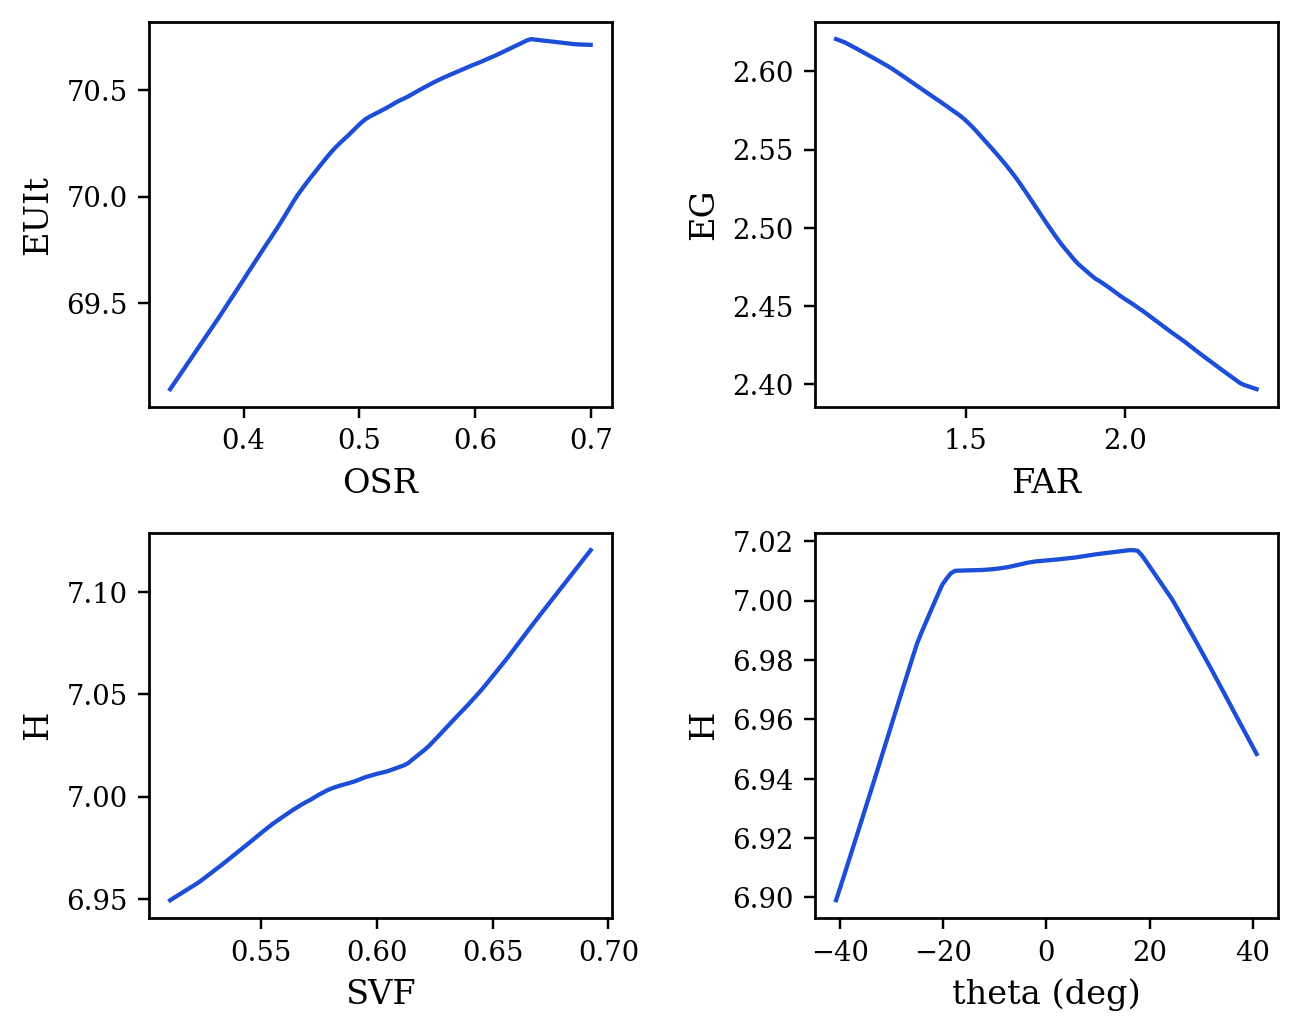
\includegraphics[width=\linewidth]{nonlinear_response_profiles.png}
\caption{Surrogate-based nonlinear response profiles for selected UMF-target pairs.}
\label{fig:supp_nonlinear}
\end{figure}

\subsection{Independent re-evaluation of selected candidates}

To reduce over-reliance on surrogate predictions, the revised workflow re-evaluates preference-aligned candidate solutions using an independent simulation call. In the current local environment, this re-evaluation still uses the fallback analytic simulator, but the code path is structured so that a full physical-stack simulation can replace it when server-side results become available. Under the current matched-checkpoint utility selection, one DDPG candidate and two NSGA-II candidates are retained after deduplication, so Table~\ref{tab:supp_reeval} reports three unique candidates. The updated comparison shows that the selected DDPG candidate undergoes much larger EUIt drift and larger EG discrepancy than the two selected NSGA-II candidates, while its H discrepancy lies between the two NSGA-II examples.

\begin{table}[H]
\centering
\caption{Independent re-evaluation of matched-checkpoint selected candidates. Surrogate and deterministic re-evaluation values are reported for the current preference-aligned selections.}
\label{tab:supp_reeval}
\begin{threeparttable}
\scriptsize
\begin{tabular}{@{}lccccccc@{}}
\toprule
Method & Scenario & EUIt$_\mathrm{sur}$ & EUIt$_\mathrm{re}$ & EG$_\mathrm{sur}$ & EG$_\mathrm{re}$ & H$_\mathrm{sur}$ & H$_\mathrm{re}$ \\
\midrule
DDPG & Generation & 66.344 & 68.342 & 2.846 & 2.724 & 7.833 & 7.646 \\
NSGA-II & NSGA-II (seed 20260310) & 66.000 & 66.000 & 2.850 & 2.828 & 7.850 & 7.676 \\
NSGA-II & NSGA-II (seed 20260328) & 66.000 & 66.000 & 2.850 & 2.738 & 7.850 & 7.622 \\
\bottomrule
\end{tabular}
\end{threeparttable}
\end{table}


\section*{Acknowledgment}

This work was supported in part by the National Natural Science Foundation of China (Grant No.~52177077), and in part by the Fundamental Research Funds for the Central Universities (Grant No.~2242023R40022).

\begin{thebibliography}{00}

\bibitem{ref1}
A. T. D. Perera, K. Javanroodi et al., ``Challenges resulting from urban density and climate change for the EU energy transition,'' \emph{Nature Energy}, vol.~8, no.~4, pp.~397--412, 2023.

\bibitem{ref2}
R. van Heerden, O. Y. Edelenbosch et al., ``Demand-side strategies enable rapid and deep cuts in buildings and transport emissions to 2050,'' \emph{Nature Energy}, vol.~10, no.~3, pp.~380--394, 2025.

\bibitem{ref3}
B. Zhou and M. Hu, ``Impact of architectural design elements on the energy efficiency and thermal comfort in neighborhood building ensembles,'' \emph{Journal of Building Engineering}, vol.~100, 2025.

\bibitem{ref4}
L. Du, H. Wang et al., ``Impact of block form on building energy consumption, urban microclimate and solar potential: A case study of Wuhan, China,'' \emph{Energy and Buildings}, vol.~328, 2025.

\bibitem{ref5}
B. Liu, Y. Liu et al., ``Urban morphology indicators and solar radiation acquisition: 2011--2022 review,'' \emph{Renewable and Sustainable Energy Reviews}, vol.~199, 2024.

\bibitem{ref6}
K. Javanroodi, A. T. D. Perera et al., ``Designing climate resilient energy systems in complex urban areas considering urban morphology: A technical review,'' \emph{Advances in Applied Energy}, vol.~12, 2023.

\bibitem{ref7}
A. T. D. Perera, K. Javanroodi, and V. M. Nik, ``Climate resilient interconnected infrastructure: Co-optimization of energy systems and urban morphology,'' \emph{Applied Energy}, vol.~285, 2021.

\bibitem{ref8}
Z. Shi, J. A. Fonseca, and A. Schlueter, ``A review of simulation-based urban form generation and optimization for energy-driven urban design,'' \emph{Building and Environment}, vol.~121, pp.~119--129, 2017.

\bibitem{ref9}
A. Eltaweel and Y. Su, ``Parametric design and daylighting: A literature review,'' \emph{Renewable and Sustainable Energy Reviews}, vol.~73, pp.~1086--1103, 2017.

\bibitem{ref10}
S. Longo, F. Montana, and E. Riva Sanseverino, ``A review on optimization and cost-optimal methodologies in low-energy buildings design and environmental considerations,'' \emph{Sustainable Cities and Society}, vol.~45, pp.~87--104, 2019.

\bibitem{ref11}
F. Ascione, R. F. De Masi et al., ``Optimization of building envelope design for nZEBs in Mediterranean climate: Performance analysis of a residential case study,'' \emph{Applied Energy}, vol.~183, pp.~938--957, 2016.

\bibitem{ref12}
G. Li, Q. He et al., ``Accelerated inverse urban design: A multi-objective optimization method to photovoltaic power generation potential, environmental performance and economic performance in urban blocks,'' \emph{Sustainable Cities and Society}, vol.~120, 2025.

\bibitem{ref13}
K. Liu, X. Xu et al., ``A multi-objective optimization framework for designing urban block forms considering daylight, energy consumption, and photovoltaic energy potential,'' \emph{Building and Environment}, vol.~242, 2023.

\bibitem{ref14}
A.-T. Nguyen, S. Reiter, and P. Rigo, ``A review on simulation-based optimization methods applied to building performance analysis,'' \emph{Applied Energy}, vol.~113, pp.~1043--1058, 2014.

\bibitem{ref15}
V. Machairas, A. Tsangrassoulis, and K. Axarli, ``Algorithms for optimization of building design: A review,'' \emph{Renewable and Sustainable Energy Reviews}, vol.~31, pp.~101--112, 2014.

\bibitem{ref16}
Y. Zhang, B. K. Teoh, and L. Zhang, ``Multi-objective optimization for energy-efficient building design considering urban heat island effects,'' \emph{Applied Energy}, vol.~376, 2024.

\bibitem{ref17}
G. Shi, S. Yao et al., ``Multi-performance collaborative optimization of existing residential building retrofitting in extremely arid and hot climate zones: A case study in Turpan, China,'' \emph{Journal of Building Engineering}, vol.~89, 2024.

\bibitem{ref18}
Y. Pan, M. Zhu et al., ``Building energy simulation and its application for building performance optimization: A review of methods, tools, and case studies,'' \emph{Advances in Applied Energy}, vol.~10, 2023.

\bibitem{ref19}
Z. Zhao, H. Li, and S. Wang, ``Surrogate-assisted coordinated design optimization of building and microclimate considering their mutual impacts,'' \emph{Applied Energy}, vol.~383, 2025.

\bibitem{ref20}
P. Westermann and R. Evins, ``Surrogate modelling for sustainable building design: A review,'' \emph{Energy and Buildings}, vol.~198, pp.~170--186, 2019.

\bibitem{ref21}
K. Li, T. Zhang, and R. Wang, ``Deep Reinforcement Learning for Multiobjective Optimization,'' \emph{IEEE Transactions on Cybernetics}, vol.~51, no.~6, pp.~3103--3114, 2021.

\bibitem{ref22}
M. Khoroshiltseva, D. Slanzi, and I. Poli, ``A Pareto-based multi-objective optimization algorithm to design energy-efficient shading devices,'' \emph{Applied Energy}, vol.~184, pp.~1400--1410, 2016.

\bibitem{ref23}
R. Liu, T. Fang et al., ``Controllable cross-building multi-objective optimisation for NZEBs: A framework utilising parametric generation and intelligent algorithms,'' \emph{Applied Energy}, vol.~374, 2024.

\bibitem{ref24}
S. Miraba, A. Salehi et al., ``Adaptive BIPV shading optimization for electricity generation and building electricity management, sDA, and DGP using multi-objective algorithms,'' \emph{Applied Energy}, vol.~402, 2025.

\bibitem{ref25}
A. Ciardiello, F. Rosso et al., ``Multi-objective approach to the optimization of shape and envelope in building energy design,'' \emph{Applied Energy}, vol.~280, 2020.

\bibitem{ref26}
X. Wang, S. Wang et al., ``Deep Reinforcement Learning: A Survey,'' \emph{IEEE Transactions on Neural Networks and Learning Systems}, vol.~35, no.~4, pp.~5064--5078, 2024.

\bibitem{ref27}
H. Jemin, L. Joonho et al., ``Learning agile and dynamic motor skills for legged robots,'' \emph{Science Robotics}, vol.~4, no.~26, 2019.

\bibitem{ref28}
O. Vinyals, I. Babuschkin et al., ``Grandmaster level in StarCraft II using multi-agent reinforcement learning,'' \emph{Nature}, vol.~575, no.~7782, pp.~350--354, 2019.

\bibitem{ref29}
X. Wang, W. Chen et al., ``Video Captioning via Hierarchical Reinforcement Learning,'' in \emph{2018 IEEE/CVF Conference on Computer Vision and Pattern Recognition (CVPR)}, 2018, pp.~4213--4222.

\bibitem{ref30}
J. Li, L. Yao et al., ``Deep reinforcement learning for pedestrian collision avoidance and human-machine cooperative driving,'' \emph{Information Sciences}, vol.~532, pp.~110--124, 2020.

\bibitem{ref31}
V. Mnih, K. Kavukcuoglu et al., ``Human-level control through deep reinforcement learning,'' \emph{Nature}, vol.~518, no.~7540, pp.~529--533, 2015.

\bibitem{ref32}
L. Timothy P, H. Jonathan J et al., ``Continuous control with deep reinforcement learning,'' \emph{arXiv preprint arXiv:1509.02971}, 2015.

\bibitem{ref33}
Y. Du, H. Zandi et al., ``Intelligent multi-zone residential HVAC control strategy based on deep reinforcement learning,'' \emph{Applied Energy}, vol.~281, 2021.

\bibitem{ref34}
S. Li, S. Su, and X. Lin, ``Optimizing the hyper-parameters of deep reinforcement learning for building control,'' \emph{Building Simulation}, vol.~18, no.~4, pp.~765--789, 2025.

\bibitem{ref35}
Z. Wu, Y. Li et al., ``Distributed voltage control for multi-feeder distribution networks considering transmission network voltage fluctuation based on robust deep reinforcement learning,'' \emph{Applied Energy}, vol.~379, 2025.

\bibitem{ref36}
P. Kou, D. Liang et al., ``Safe deep reinforcement learning-based constrained optimal control scheme for active distribution networks,'' \emph{Applied Energy}, vol.~264, 2020.

\end{thebibliography}


\end{document}
